\section{Approach}
\label{sec:approach}

We next describe our approach, called TeMAPI, that accepts two tools as inputs: a translation tool under analysis and a test-generation tool. TeMAPI effectively leverages the test-generation tool to generate test cases that detect behavioral differences of API mapping relations defined by the translation tool. TeMAPI addresses two major issues in detecting behavioral differences of API mapping relations. First, it is challenging to extract API mapping relations defined by the translation tool. The primary reason is that often translation tools either use different formats for specifying API mapping relations or do not explicitly describe these mapping relations. In the later case, API mapping relations are hard coded within the source code of translation tools such as Sharpen. To address this issue and to be independent of the translation tool under analysis, TeMAPI does not extract API mapping relations directly from translation tools. Instead, TeMAPI analyzes translated code for extracting those relations. In particular, TeMAPI constructs \emph{wrapper} methods for each API element in a language and translates those wrapper methods to another language to extract the API mapping relations. Section~\ref{sec:approach:wrapper} presents more details on how wrapper methods are constructed from API elements. These wrapper methods also help identify the API elements that can be translated by the translation tool under analysis, since often translation tools translate only a limited set of API elements~\cite{zhong2010mining}.

Second, exposing behavioral differences among API elements that are defined by API mapping relations poses testability issues. For example, interface of an API method in one language could be different from the interface of its mapped API method or an API method in one language can be mapped to multiple API methods in the other language, resulting in controllability issues. On the other hand, generating test oracles is also challenging, resulting in observability issues. TeMAPI addresses these issues by using wrapper methods as an abstraction. In particular, these wrapper methods expose a common interface for API elements that are defined by API mapping relations, thereby addressing controllability issues. Furthermore, to address observability issues, TeMAPI uses return values of wrapper methods or exceptions being thrown as test oracles. We next describe more details on how wrapper methods are constructed and later describe how TeMAPI leverages two existing state-of-the-art test-generation techniques Pex~\cite{tillmann2008pex} and Randoop~\cite{pacheco2007feedback} for generating test cases that detect behavioral differences. In our approach, we use Pex and Randoop, since both these test-generation tools are popular and are shown to be effective in detecting serious defects in industrial code bases. Furthermore, Pex is effective in generating data for primitive types and Randoop is effective in generating method sequences by combining method calls randomly, complementing each other. However, TeMAPI is general and any other test-generation tool such as Java PathFinder~\cite{DBLP:conf/tacas/AnandPV07} can be easily leveraged to generate test cases due to the abstraction provided by the wrapper methods.

\Comment{
\begin{figure}[t]
\centering
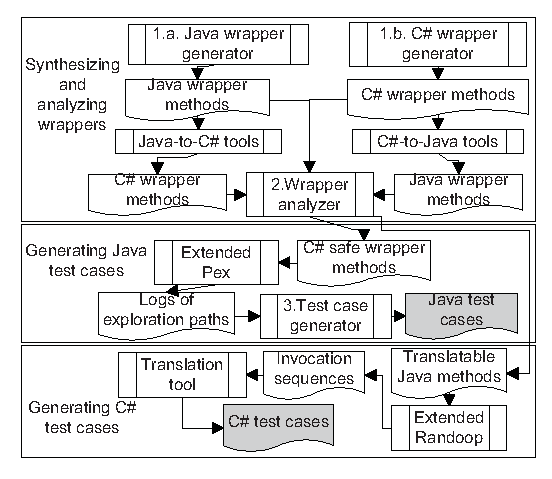
\includegraphics[scale=1,clip]{figure/approach.eps}\vspace*{-2ex}
 \caption{Overview of TeMAPI}\vspace*{-2ex}
 \label{fig:approach}
\end{figure}

As shown in Figure~\ref{fig:approach}, given a translation tool between Java and C\#, TeMAPI generates various test cases in Java and C\# to reveal behavioral differences of API mapping relations defined by the tool.}

%-------------------------------------------------------------------
\subsection{Synthesizing and Analyzing Wrappers}
\label{sec:approach:wrapper}

Given a translation tool under analysis, TeMAPI first extracts its API mapping relations. To deal with different formats of translation tools as described in Section~\ref{sec:introduction}, TeMAPI does not extract API mapping relations directly from translation tools, but analyzes translated code for such relations. TeMAPI includes a wrapper generator that generates wrappers for API elements in both Java and C\#. For static fields and static methods, the two wrapper generators of TeMAPI use the following rules to synthesize wrapper methods. In the synthesized code below, ``\CodeIn{|f.name|}'' denotes the name of a field \CodeIn{f}; ``\CodeIn{|m.name|}'' denotes the name of a method \CodeIn{m}; and ``\CodeIn{|no|}'' denotes the id of the synthesized wrapper method.

\textbf{Static fields.} Given a public static field \CodeIn{f} of a class \CodeIn{C} whose type is \CodeIn{T}, TeMAPI synthesizes a getter as follows:

\begin{CodeOut}%\vspace*{-1.5ex}
\begin{alltt}
 public T testGet|f.name||no|sfg()\{ return C.f; \}
\end{alltt}
\end{CodeOut}%\vspace*{-1.5ex}

If \CodeIn{f} is not a constant, TeMAPI synthesizes a setter as follows:

\begin{CodeOut}%\vspace*{-1.5ex}
\begin{alltt}
 public void testSet|f.name||no|sfs(T v)\{ C.f = v; \}
\end{alltt}
\end{CodeOut}%\vspace*{-1.5ex}

\textbf{Static methods.} Given a public static method \CodeIn{m(T1\ m1,\ldots,Tn\ mn)} of a class \CodeIn{C} whose return type is \CodeIn{Tm}, TeMAPI synthesizes a wrapper method as follows:

\begin{CodeOut}%\vspace*{-1.5ex}
\begin{alltt}
 public Tm test|m.name||no|sm(T1\ m1,\ldots, Tn\ mn)\{
   return C.m(m1,\ldots, mn);
 \}
\end{alltt}
\end{CodeOut}%\vspace*{-1.5ex}

When TeMAPI synthesizes wrapper methods for non-static fields or methods, TeMAPI takes constructors into considerations.

\textbf{Non-static fields.} Given a public non-static field \CodeIn{f} of a class \CodeIn{C} whose type is \CodeIn{T}, TeMAPI synthesizes a getter using each constructor \CodeIn{C(T1\ c1,\ldots, Tn\ cn)} of \CodeIn{C} as follows:

\begin{CodeOut}%\vspace*{-1.5ex}
\begin{alltt}
 public T testGet|f.name||no|nfg(T1\ c1,\ldots, Tn\ cn)\{
    C obj = new C(c1,\ldots, cn);
    return obj.f;
 \}
\end{alltt}
\end{CodeOut}%\vspace*{-1.5ex}

If \CodeIn{f} is not a constant, TeMAPI synthesizes a setter as follows:

\begin{CodeOut}%\vspace*{-1.5ex}
\begin{alltt}
 public void testSet|f.name||no|nfs(T v, T1\ c1,\ldots, Tn\ cn)\{
   C obj = new C(c1,\ldots, cn);
   obj.f = v;
 \}
\end{alltt}
\end{CodeOut}%\vspace*{-1.5ex}

\textbf{Non-static methods.} Given a public non-static method \CodeIn{m(T1\ m1,\ldots,Tn\ mn)} of a class \CodeIn{C} whose return type is \CodeIn{Tm}, TeMAPI synthesizes a wrapper method using each constructor \CodeIn{C(Tv\ cv,\ldots, Tt\ ct)} of \CodeIn{C} as follows:

\begin{CodeOut}%\vspace*{-1.5ex}
\begin{alltt}
 public Tm test|m.name||no|nm(T1\ m1,\ldots, Tn\ mn, Tv cv, \ldots, Tt ct)\{
   C obj = new C(cv,\ldots, ct);
   return obj.m(m1,\ldots, mn);
 \}
\end{alltt}
\end{CodeOut}%\vspace*{-1.5ex}


TeMAPI groups all synthesized wrapper methods for one API class $C$ to one synthesized class. When synthesizing, TeMAPI ignores generic methods, since the translation tools cannot handle generics. Furthermore, when synthesizing wrappers for C\# API classes, TeMAPI ignores \CodeIn{unsafe} methods, \CodeIn{delegate} methods, and methods whose parameters are marked as \CodeIn{out} or \CodeIn{ref} besides generic methods. Java does not have these corresponding keywords, so existing translation tools typically do not translate the preceding methods. After wrapper methods are synthesized, TeMAPI uses the translation tool under analysis to translate wrapper methods to the other language.

Our synthesized wrappers are quite simple in their structures. Therefore, existing translation tools are typically able to translate their structures correctly. Still, some translated wrappers can have compilation errors, since existing translation tools cannot translate some API elements. We use \emph{safe wrappers} to refer to the wrappers that are translated without compilation errors. To identify safe wrappers, TeMAPI extends Visual Studio and Eclipse's Java compiler for C\# and Java code, respectively. Comparing source code of safe wrappers with source code of synthesized wrappers, TeMAPI extracts one-to-one mapping relations of API classes for the tool under analysis. For example, by comparing the first statements of the \CodeIn{testskip24nm} method in Java and in C\# as shown in Section~\ref{sec:example}, TeMAPI extracts the mapping relation between the \CodeIn{ByteArrayInputStream} class in Java and the \CodeIn{MemoryStream} class in C\# defined by JLCA. Through analysis, TeMAPI also extracts translatable API methods for the translation tool under analysis. In the preceding example, TeMAPI adds \CodeIn{BufferedInputStream(InputStream)} constructor and the \CodeIn{skip(long)} method in Java to translatable API methods of JLCA, since their belonging wrapper method is translated from Java to C\# without compilation errors.

%--------------------------------------------------------
\subsection{Generating Test Cases using Pex}
\label{sec:approach:single}

We next describe how TeMAPI generates test cases that detect behavioral differences using Pex. Pex uses a technique, called dynamic symbolic execution~\cite{koushik:cute, godefroid:dart}, for systematically exploring the code under test and generates test cases that exercise various paths in the code under test. In particular, TeMAPI applies Pex on safe wrappers in C\# language, since Pex handles .NET code. A primary advantage of wrappers is that wrappers provide the same interface for both C\# and Java versions and abstracts the details of API elements within the wrapper method. We next explain how TeMAPI generates test cases for Java to C\# and C\# to Java translation tools and present the technical challenges addressed by TeMAPI.

To generate test cases for Java to C\# translation tools, TeMAPI synthesizes wrappers in Java and translates those wrappers into C\#. TeMAPI next generates test cases on wrappers in C\# using Pex. TeMAPI captures the return values of wrapper methods or exceptions being thrown and uses them as test oracles in generated test cases. TeMAPI next translates generated test cases to Java to detect behavioral differences. On the other for C\# to Java translation tools, TeMAPI synthesizes wrappers in C\# and generates test cases on those wrappers. TeMAPI next translates both synthesized wrapper methods and generated test cases to Java to detect behavioral differences.

%Wrappers are beneficial to detect behavioral differences for two factors. (1) Wrapper methods expose all the inputs of their wrapped methods and constructors, so it is feasible to change values of the inputs to exercise their paths. (2) Each wrapper method has one constructor and one method at most, so it is easy to locate which method has behavioral differences. Due to the two factors, TeMAPI extends Pex~\cite{tillmann2008pex} to generate test cases for safe wrappers for each API class in C\#. For each safe wrapper, TeMAPI leverages Pex to explore feasible paths among API methods within wrappers. When exploring, TeMAPI records the inputs and the corresponding output of each unique feasible path to generate a test case. As each path is unique, each test case reflects a unique behavior. 

We next describe the technical challenges addressed by TeMAPI while translating test cases generated in C\# to Java. When translating test cases to Java, TeMAPI refers to the extracted mapping relations of API elements (Section~\ref{sec:approach:wrapper}) to translate C\# values into Java values. In a few cases, values of some primitive types can cause compilation errors. Therefore, TeMAPI replaces them with corresponding method invocations. For example, the \CodeIn{long m0 = 2147483648} statement causes a compilation error with a message: ``The literal 2147483648 of type \CodeIn{int} is out of range''. In Section~\ref{sec:example}, TeMAPI uses a method invocation to replace this statement in the \CodeIn{testskip24nm} test case. Pex includes some heuristics for generating data factories for non-primitive types\footnote{In our future work, we plan to further enhance these data factories using our previous work~\cite{thummalapenta09:mseqgen}.}. For these non-primitive types, TeMAPI refers to extracted mapping relations of API elements to translate them. To check equivalence of outputs, TeMAPI checks whether their values are equal for primitive types and arrays, and checks whether each mapped field is equal for objects. For example, TeMAPI records that given an empty object, the \CodeIn{testappend175nm} wrapper method in C\# returns a \CodeIn{StringBuilder} object whose \CodeIn{Capacity} field is 16 and \CodeIn{Length} field is 13, so TeMAPI derives a test case for the corresponding Java wrapper method as follows:

\begin{CodeOut}%\vspace*{-1.5ex}
\begin{alltt}
public void testappend175nm122()\{
  Test_java_lang_StringBuffer obj = new Test_java_lang_StringBuffer();
  Object m0 = new Object();
  StringBuffer out = obj.testappend175nm(m0);
  Assert.assertEquals(16, out.capacity());	
  Assert.assertEquals(13, out.length());
\}
\end{alltt}
\end{CodeOut}%\vspace*{-2ex}

This test case fails, since here the \CodeIn{capacity()} method returns 34 and the \CodeIn{length()} method returns 24. Thus, TeMAPI detects two behavioral differences between the \CodeIn{java. lang.StringBuffer} class in Java and the \CodeIn{System.Text.StringBuilder} class in C\#. 

%Since our wrapper methods use fixed invocation sequences, they also help in addressing the issue of generating sequences with Pex~\cite{thummalapenta09:mseqgen}.

We notice that when Pex explores a path with some specific inputs, the method under exploration throws exceptions.
For example, during exploring the \CodeIn{testvalueOf61sm} wrapper method in C\#, TeMAPI records that given a \CodeIn{null} input, the method throws \CodeIn{NullReferenceException}, so TeMAPI derives a test case to ensure that the corresponding Java wrapper method also throws a mapped exception. To derive the test case, TeMAPI finds the corresponding exceptions in Java by analyzing translated wrapper methods with synthesized ones. In this example, TeMAPI finds that the \CodeIn{NullReference- Exception} class in C\# is mapped to the \CodeIn{NullPointerException} class in Java with respect to the API mapping relations of Java2CSharp, so TeMAPI derives a Java test case as follows:

\begin{CodeOut}\vspace*{-1.5ex}
\begin{alltt}
 public void testvalueOf61sm3()\{
   try\{
     Test_java_lang_String obj = new Test_java_lang_String();
     java.lang.Object m0 = null;
     obj.testvalueOf61sm(m0);
   \}catch(java.lang.NullPointerException e)\{
     Assert.assertTrue(true);
     return;
   \}
   Assert.assertTrue(false);
 \}
\end{alltt}
\end{CodeOut}\vspace*{-1ex}

This test case gets failed since the \CodeIn{testvalueOf61sm} method in Java does not throw any exceptions given a null input.
From this failing test case, TeMAPI detects the behavioral difference between the \CodeIn{java.lang.String.valueOf(Object)} method in Java and the \CodeIn{System.Object.ToString()} method in C\#, since the two wrapper methods invoked by the two preceding test cases are for these two API methods. When the translation tool under analysis is from C\# to Java, wrapper methods generated for C\# are used for deriving C\# test cases for Java code.

%-----------------------------------------------------------
\subsection{Generating Test Cases using Randoop}

\label{sec:approach:sequence}
\begin{table}[t]
\centering
\begin{SmallOut}
\begin {tabular} {|c|l|c|c|c|c|c|c|}
\hline
\textbf{Name}& \textbf{Version}& \textbf{Provider} &\textbf{Description}\\
\hline
Java2CSharp  &  1.3.4 & IBM (ILOG) & a Java-to-C\# translation tool\\
\hline
JLCA         &  3.0   & Microsoft  & a Java-to-C\# translation tool\\
\hline
sharpen      &  1.4.6 & db4o       & a Java-to-C\# translation tool \\
\hline
Net2Java     &  1.0   & NetBean    & a C\#-to-Java translation tool\\
\hline
converter    &  1.6   & Tangible   & a C\#-to-Java translation tool\\
\hline
\end{tabular}%\vspace*{-2ex}
\Caption{Subject tools} \label{table:subjects}
\end{SmallOut}\vspace*{-4ex}
\end{table}

Despite of its benefits to detect behavioral differences, a wrapper method cannot help effectively generate test invocation sequences, since it has fixed invocation sequences (\emph{e.g.}, a constructor first and then the public method). To address this issue, TeMAPI extends Randoop~\cite{pacheco2007feedback} for Java to generate invocation sequences in Java for all translatable API methods of the translation tool under analysis. Randoop randomly generates test cases based on already generated test cases in a feedback-directed manner. In particular, when using Randoop to generate test cases, TeMAPI limits its search scope to translatable API methods. TeMAPI runs generated test cases, and removes all failing test cases. TeMAPI next uses the translation tool under analysis to translate generated Java test cases to the other language C\#. If translated code has the same behaviors, translated test cases should also get passed. If not, TeMAPI detects behavioral differences. Randoop-generated Java test cases also include \CodeIn{assert} statements to assert behaviors of Java code. Thus, TeMAPI does not need to generate assertion statements as it does with Pex. Section~\ref{sec:evaluation:sequence} shows such detected behavioral differences that are related to invocation sequences (\emph{e.g.}, the \CodeIn{test423} test cases).

%As the inputs and outputs between Randoop and Pex are both different, TeMAPI is asymmetric when generating test cases in Java and in C\# as shown in Figure~\ref{fig:approach}. 

%NOTE: TeMAPI filters out failing tests of Randoop but not the failing tests of Pex, which is inconsistence. The next version should fix this issue 